\cotefile{74}
\scanpage{121}
% archive sheet number: 120
\margin{$c=2^{\unsure{\nu|\omega}}$}
\diagram{\resizebox{\linewidth}{!}{$\begin{array}{ll|c|c|c|c}
&&c=0&1&2&4\\ \hline
\text{Nb de triangles incidents à un \unsure{sommet}}:&c+1=e&1&2&3&5\\ \hline
\text{Nb de sommets}\quad\text{--- --- ---}:&2(c+1)&2&4&6&10\\ \hline
\text{Nb de sommets}:&3(1+2c)=3+6c&3&9&15&27\\ \hline
\text{Nb des \deleted{triangles}\inserted{arêtes}}:&\begin{gathered}3(c+1)(1+2c)\deleted{\unsure{=3(1}}\\=3(1+3c+2c^2)\end{gathered}&3&18&45&135\\ \hline
\text{Nb de triangles}&(c+1)(1+2c)=1+3c+2c^2&1&6&15&45\\ \hline
\text{\uline{Nb de triangles}}&\text{verticaux}=3c&0&3&6&12\\ \cline{2-6}
&\begin{gathered}\text{transversaux}\quad 2c^2\\=2\;2^{2\nu}=2^{2\nu+1}\quad(\nu=-\infty,0,1,2)\end{gathered}&0&2&8&32\\ \hline
\text{NB de sommets antiliés à un sommet}&4c=2^{\nu+\unsure{2}}&0&\begin{gathered}4=2^2\\=2^e\end{gathered}&\begin{gathered}8=2^3\\=2^e\end{gathered}&\begin{gathered}16=2^4\\=2^{e-1}\end{gathered}\\ \hline\hline
\text{Ordre de }\operatorname{Aut}(S,A):\quad N_{\omega}&&6=2.3&72=2^3.3^2&\unsure{720|360}=2^{\unsure{4}}.3^2.5&51840=2^7\,3^4\,5\\ \hline\hline
\text{Nb de }\mathcal T_{\deleted{\unsure{0}}-1}\ \text{(\unsure{triangle|triangles}) plongés}&(c+1)(2c+1)=1+3c+\unsure{c^2|2|2c^2}&1&6=2.3&15=3.5&45=3^2.5\\ \hline
\begin{gathered}\text{Nb de }\mathcal T_0\ \text{(\unsure{bitriangle|bitriangles}) plongés)}\\ \deleted{\text{si }c=2^\nu\quad\nu=1,2}\end{gathered}&\deleted{\unsure{(c+1)}}\ \frac16\deleted{\unsure{c}}c(c+1)(2c+1)&0&1&10&\begin{gathered}120\\\deleted{\unsure{2^3.3.5}}\end{gathered}\\ \hline
\text{Nb de }\mathcal T_1\ \text{(\unsure{tritriangle|tritriangles}) plongés}&\frac{1}{30}c(c+1)(2c+1)(c-1)&0&0&1&\unsure{36}=2^2 3^2\\ \hline\hline
&&6&\unsure{36}=2^2 3^2&90=2.3^2.5&270=2.3^3.5\\ \cline{3-6}
\multicolumn{2}{l|}{\text{comme trois figures précédentes, mais avec \unsure{strs|des} \uline{\unsure{cplt figées|$c\geq1$ épinglés}}}}&0&72=2^3.3^2&\begin{gathered}360=\\2^{3}.3^2.5\end{gathered}&\begin{gathered}\inserted{2160}\\\deleted{\unsure{2160}}=\\2^{\unsure{6|4}}.3^{\unsure{3}}.5\end{gathered}\\ \cline{3-6}
&&0&0&720=2^4.3^2.5&2^6.3^4.5\\ \cline{3-6}
&&0&0&0&2^7.3^4.5\\ \cline{3-6}
\end{array}$}}
\scanpage{122}
% archive sheet number: 121 (inverted, at the upper right)
\diagram{\begin{tikzcd}[ampersand replacement=\&,row sep=small]
\unsure{\cdot}\arrow[dr,dashed,no head]\& \& \unsure{\cdot|1}\\
\& V\arrow[r,"\varphi_i"]\arrow[dr,dashed,"\psi_i"']\& \Gamma\arrow[u]\arrow[rr,"p_i","\deleted{\unsure{\sim}}"']\& \& \deleted{\unsure{E/|E/2}}_{i}=V\\
\& \& \widetilde\Gamma\arrow[u]\arrow[dr,"\widetilde p_i"]\\
\& \& \{\pm1\}\arrow[u]\&\widetilde E_i\arrow[uur]\\
\& \& \unsure{?|0}\& \pm1\arrow[ul]\arrow[u]\\
\& \widetilde\Gamma\arrow[r]\&\widetilde E_i
\end{tikzcd}}
\[
\begin{aligned}
&x\quad y\quad z\\
&x\quad\underline{y+u+\unsure{w|v}},\quad\underline{z+u+w}\\
&\phantom{x}\quad x_0\quad y_0+w\quad z_0+w\\
&\deleted{x\quad y\quad z}\\
&\deleted{x\quad z+\unsure{u}\quad y+}
\end{aligned}
\]
\[
\begin{aligned}
&g\in\widetilde E_1=V\\
&\widetilde y\in\widetilde E_2
\end{aligned}
\]
\diagram{\begin{tikzcd}[ampersand replacement=\&,row sep=tiny]
\&\& \unsure{3|\ni}\arrow[d]\\
0\arrow[r]\&\widetilde\Gamma\arrow[r,leftrightarrow]\&\widetilde E_1\times\widetilde E_2\arrow[r]\& {} \&\widetilde\Gamma\arrow[r,no head]\&E_2\\
\&\&\deleted{(g,y)}\quad\varepsilon
\end{tikzcd}}
\diagram{\begin{tikzcd}[ampersand replacement=\&,column sep=small]
s\arrow[r]\&t'\arrow[r]\&u\arrow[r]\&s'
\end{tikzcd}}
\diagram{\begin{tikzcd}[ampersand replacement=\&]
\widetilde\Gamma\arrow[d,"\widetilde p_3"']\arrow[r,phantom,"\simeq"]\&E_1\times\widetilde E_2\arrow[r]\arrow[dl,"q_{12}"']\&E_1\times E_2\arrow[dl]\\
\widetilde E_3\arrow[r,"\deleted{\unsure{\leftarrow}}"']\arrow[d]\&E_3\\
\deleted{\unsure{E_3}}
\end{tikzcd}}
\diagram{\begin{tikzcd}[ampersand replacement=\&,row sep=small]
\&(x,y)\arrow[dl,mapsto]\\
\unsure{x+y|x*y}\quad(=-x-y)
\end{tikzcd}}
\[
\begin{aligned}
q_{12}(a.\widetilde y)&=q_{1\unsure{2|\varepsilon}}(a)\,q_{12}\unsure{(|\widetilde y}\\
2^4/2&=2^2
\end{aligned}
\]
\[
\begin{aligned}
&\deleted{\sigma_1\quad\sigma_2\quad\sigma_3}\\
&\tau_1\quad\tau_2\quad\tau_3
\end{aligned}
\]
\diagram{\begin{tikzcd}[ampersand replacement=\&,row sep=small,column sep=small]
\& E'\&\\
E\arrow[ur,"\tau_3"]\arrow[rr,no head,"\tau_2"']\&\&\unsure{E''|E_2|\widetilde E_2}\arrow[ul,"\tau_1"]
\end{tikzcd}}
\[
\begin{aligned}
&\tau_2\tau_1=\mathrm{id}\qquad\tau_3\tau_2=\mathrm{id}\qquad\tau_1\tau_{2}=\mathrm{id}\\
&\tau^2=\mathrm{id}
\end{aligned}
\]
\[
\begin{aligned}
&\widetilde G\quad\text{sur}\quad\widetilde\Gamma\\
&\sigma_x\sigma_y\sigma_x^{-1}\sigma_y^{-1}\\
&=\sigma_{\underbrace{\sigma_x y}_{z}}\ \sigma_{\unsure{\cdot\cdot|y}}
\end{aligned}
\]
\[
\widetilde\Gamma\subset\widetilde E^3
\]
\[
\underbrace{\sigma_x\sigma_{x'}}_{\pi}\ \underbrace{\sigma_y\sigma_{y'}}_{\sigma_{\pi y}\,\sigma_{\pi y'}}\
\sigma_x\sigma_{x'}\sigma_y\sigma_{y'}\qquad
\pi_{x,x'}\pi_{y,y'}=\pi_{x,x'}\pi_{\pi_{\unsure{x,x'}}y,\unsure{\pi}}
\]
\scanpage{123}
% archive sheet number: 122
% printed form
N\textsuperscript{o}\hfill ACADEMIE DE MONTPELLIER

UNIVERSITÉ DES SCIENCES ET TECHNIQUES DU LANGUEDOC

\textit{Examen de}\textsuperscript{ (1)} \dotfill

\noindent\dotfill

\textit{Nom et Prénoms du Candidat}\textsuperscript{ (2)} \dotfill

\textit{né à} \dotfill\quad \textit{département de} \dotfill

\textit{le} \dotfill\quad 19

\textit{Montpellier, le} \dotfill\quad 19

COMPOSITION EN \dotfill

(1) -- Le candidat doit indiquer la nature de l'examen auquel il se présente.

(2) -- Le candidat inscrit ses nom, prénom, lieu et date de naissance en tête de la copie et signe lisiblement son nom à la fin de la composition.

% margin note written sideways
\margin{\handwritten{$\begin{gathered}
12.4^2\deleted{\unsure{8|6}}.9.5=2^6.3^3.5\\
\underline{2^7}.3^4.5\ \big|\ 2.3\\[-2pt]
\begin{array}{r}
128\\640\\\unsure{81|87}\\\hline
640\\\unsure{5120|3120}\\\hline
51.840
\end{array}
\end{gathered}$}}
\scanpage{124}
% archive sheet number: 123
\[
\begin{aligned}
\deleted{\unsure{\mathcal T|\tau}}\ \mathcal T_{-2}&\quad\text{graphe vide}\\
\mathcal T_{-1}&\quad\text{graphe \deleted{\unsure{vide}} triangle}\qquad c=0=2^{-\infty}\\
\mathcal T_0&\quad\text{--- \deleted{\unsure{bitriangle}}\inserted{pavé}}\qquad c=1=2^0\\
\mathcal T_1&\quad\text{---}\qquad c=2=2^1\\
\mathcal T_2&\quad\text{``\unsure{graphe|graphes}'' cubique}\qquad c=4=2^2
\end{aligned}
\]

Cat. des graphes $\mathcal T_\alpha$ munis d'une \unsure{sous-structure|sgstructure} $\mathcal T_\beta$ $(\beta\leq\alpha)$
\diagram{\resizebox{\linewidth}{!}{$\begin{array}{c|c|c|c|c}
\beta\backslash\alpha&-1&0&1&2\\\hline
\unsure{-\varnothing|-2|-\infty}&(\mathrm{Ens})_3&(\mathrm{Ens})_{3,3}&(\mathrm{Ens})_6&*\\
-1&(\mathrm{Ens})_3&(\mathrm{Ens})_3\times(\mathrm{Ens})_2&(\mathrm{Ens})_{2,2,2}\deleted{\unsure{\mathrm{trans}}}&\text{Trialité}\\
0&\varnothing&(\mathrm{Ens})_{3,3}&(\mathrm{Ens})_{3,3}&(\mathrm{Ens})_{\unsure{3,3}}\times(\mathrm{Ens})_{3,3}\\
\deleted{\unsure{4|1}}1&\varnothing&\varnothing&(\mathrm{Ens})_6&(\mathrm{Ens})_6\times(\mathrm{Ens})_2\\\hline
\end{array}$}}
Cat des systèmes $\mathcal T_\alpha\subset\mathcal T_\beta\subset\mathcal T_\gamma$\quad $(\underset{\substack{\Vert\\-2}}{\alpha}<\beta<\gamma\ \text{fixés})$
\[
\unsure{\text{ou}}\quad\mathcal T_{-1}\subset\mathcal T_0\unsure{\subset}\mathcal T_1\subset\mathcal T_2
\]
\diagram{$\begin{array}{r|l}
-1,0,1&(\mathrm{Ens})_3\\\hline
-1,0,2&(\mathrm{Ens})_3\times(\mathrm{Ens})_3\\\hline
-1,1,2&(\mathrm{Ens})_{2,2,2}\times(\mathrm{Ens})_2\\\hline
0,1,2&(\mathrm{Ens})_{3,3}\times(\mathrm{Ens})_2\\\hline
-1,0,1,2&(\mathrm{Ens})_3\times(\mathrm{Ens})_2
\end{array}$}

\margin{$\unsure{r\,p^{=}|rp^e}$}
\scanpage{125}
% archive sheet number: 124
\[
\begin{aligned}
\sigma_{t_0}:&\quad x\leftrightarrow x',\quad y\leftrightarrow y',\quad z\leftrightarrow z'\\
\sigma_{t\deleted{\unsure{'}}}:&\quad x\leftrightarrow y',\quad y\leftrightarrow z',\quad z\leftrightarrow x'\\
\sigma_{t'}:&\quad x\leftrightarrow z',\quad y\leftrightarrow x',\quad z\leftrightarrow y'
\end{aligned}
\]
\diagram{\resizebox{\linewidth}{!}{\begin{tikzcd}[ampersand replacement=\&,column sep=small,row sep=large]
\sigma_{t_0}\sigma_t: \&x\arrow[r]\&\deleted{\unsure{z}}y\arrow[r]\&\deleted{\unsure{y}}z\arrow[ll,bend right=35]\&x'\arrow[r]\&z'\arrow[r]\&y'\arrow[ll,bend right=35]\&a\arrow[r]\&s\arrow[r]\&s'\arrow[ll,bend right=35]\\
\Vert\&\&\deleted{\unsure{y\longmapsto x}}\\[-1ex]
\sigma_t\sigma_{t'}:\&x\arrow[r]\&y\arrow[r]\&z\arrow[ll,bend right=35]\&x'\arrow[r,no head]\&\unsure{z'}\arrow[r,no head]\&y'\arrow[ll,bend right=35]\&a\arrow[r]\&s\arrow[r]\&s'\arrow[ll,bend right=35]\\
\Vert\\
\sigma_{t'}\sigma_{t_0}:\&\&\&\&\mathrm{id}
\end{tikzcd}}}
\[
\begin{aligned}
&\sigma_{t_0}\sigma_t=\sigma_t\sigma_{t'}=\sigma_{t'}\sigma_{t_0}\deleted{\unsure{=[\sigma_{t_0},\sigma_t]}}=\pi_{a},\quad\pi^3=\mathrm{id}\\
\Downarrow\quad&[\sigma_{t_0},\sigma_t]=[\sigma_t,\sigma_{t'}]=[\sigma_{t'},\sigma_{t_0}]=\pi^2=\pi^{-1})\\
&\sigma_t\sigma_{t_0}=\sigma_{t_0}\sigma_{t'}=\sigma_{t'}\sigma_t=\pi^{-1}\\
\mathrel{\swarrow\!\!\swarrow}\quad&\deleted{\unsure{\sigma_t}}\sigma_{t_0}\sigma_t\sigma_{t'}=\sigma_t\quad\text{etc}
\end{aligned}
\]

$\unsure{\mathfrak S|\mathcal S|\mathcal G}_I$ opère sur $S\unsure{\smallsetminus|-}\underbrace{X}_{\substack{\text{bitriangle}\\\text{plongé}}}$, sans pt fixe (\unsure{orbites}\ \unsure{à} 6 \unsure{élmts}) et \unsure{---} trois orbites, donc trois torseurs sous $\mathfrak S_I$ donc trois ens à trois éléments

\figure{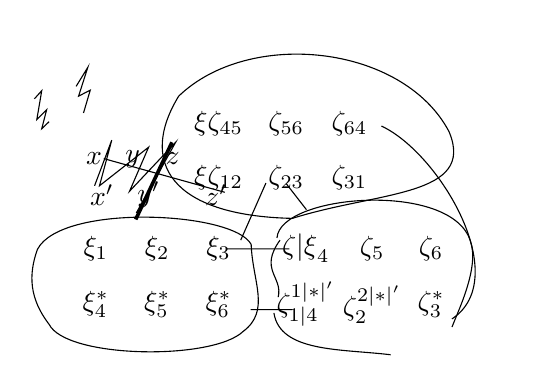
\begin{tikzpicture}[x=.78cm,y=.69cm,every node/.style={inner sep=1pt}]
\draw (2.35,4.45) .. controls (3.5,5.7) and (6.0,5.4) .. (6.75,3.8) .. controls (7.2,2.6) and (5.6,2.7) .. (4.2,2.2) .. controls (2.2,2.25) and (1.7,3.25) .. (2.35,4.45);
\draw (3.95,1.84) .. controls (4.0,2.65) and (6.8,2.9) .. (7.1,1.78) .. controls (7.25,1.3) and (6.9,.5) .. (6.8,.2);
\draw (4.0,1.8) .. controls (3.65,1.25) and (4.05,1.13) .. (3.97,.75);
\draw (3.9,.46) .. controls (4.0,-.27) and (5.0,-.2) .. (5.8,-.31);
\draw (.05,1.63) .. controls (.44,2.48) and (3.25,2.33) .. (3.53,1.72) .. controls (3.55,1.04) and (3.85,.5) .. (3.4,.12) .. controls (2.9,-.42) and (.52,-.38) .. (.24,.25) .. controls (-.08,.72) and (-.1,1.16) .. (.05,1.63);
\foreach \x/\a/\b in {1/1/4,2/2/5,3/3/6}{\node at (\x,1.65){$\xi_{\a}$};\node at (\x,.62){$\xi_{\b}^{*}$};}
\node at (4.42,1.65){$\unsure{\zeta|\xi}_4$};\node at (5.5,1.65){$\zeta_5$};\node at (6.46,1.65){$\zeta_6$};
\node at (4.42,.62){$\zeta_{\unsure{1|4}}^{\unsure{1|*|'}}$};\node at (5.5,.62){$\zeta_2^{\unsure{2|*|'}}$};\node at (6.46,.62){$\zeta_3^{*}$};
\node at (3,3.95){$\deleted{\unsure{\xi}}\zeta_{45}$};\node at (4.1,3.95){$\zeta_{56}$};\node at (5.13,3.95){$\zeta_{64}$};
\node at (3,2.96){$\deleted{\unsure{\xi}}\zeta_{12}$};\node at (4.1,2.96){$\zeta_{23}$};\node at (5.13,2.96){$\zeta_{31}$};
\draw (3.12,1.64)--(4.15,1.64) (3.52,.52)--(4.2,.52) (3.36,1.8)--(3.77,2.85) (4.1,2.84)--(4.43,2.36);
\draw (5.65,3.9) .. controls (6.6,3.4) and (7.8,1.1) .. (6.8,.35);
\node at (.97,3.3){$x$};\node at (1.6,3.28){$\deleted{\unsure{y}}$};\node at (2.25,3.3){$\deleted{\unsure{z}}$};
\node at (1.1,2.63){$x'$};\node at (1.86,2.63){$y'$};\node at (2.96,2.63){$z'$};
\draw (.98,2.8)--(1.26,3.64)--(1.06,2.8)--(1.86,3.51)--(1.55,2.7)--(2.3,3.6)--(1.66,2.3) (1.13,3.3)--(3.1,2.68);
\draw[line width=1.3pt] (1.65,2.18)--(2.24,3.6);
\draw (.0,4.4)--(.12,4.55)--(.04,4.02)--(.2,4.2)--(.12,3.85)--(.24,3.98) (.68,4.63)--(.87,4.98)--(.72,4.45)--(.91,4.56)--(.8,4.14);
\end{tikzpicture}}
\diagram{\begin{tikzcd}[ampersand replacement=\&]
\deleted{X}\arrow[d]\&Z\arrow[d]\&\text{ens à 9 él.}\\
{}\&E\&\text{ens à 3 él.}
\end{tikzcd}}

$I,J$ deux ens à trois él.

$\mathfrak S_I\times\mathfrak S_J$ opère sur ens \deleted{à 18} fini, \inserted{$E$} \deleted{de} façon que $\mathfrak S_I$ et $\mathfrak S_J$ opèrent ss pts fixes, donc \unsure{---} $E=\coprod E_i$, chaque $E_i$ bitorseur sous $\mathfrak S_{\unsure{i|I}}\times\mathfrak S_J$
\scanpage{126}
% archive sheet number: 125
\margin{$\begin{aligned}&\deleted{3(1+2c)}\\&\tfrac12(3+6c)(2+2c)\\&=3(1+2c)(1+c)\\&=3(1+3c+2c^2)\end{aligned}$}
\[
\begin{aligned}
&(a\quad b\quad c)\\
&\deleted{\unsure{x\in\widetilde E_a\quad x}}\\
&(\unsure{s|1},t,u)\qquad (s',t',u')\\
&x\in E_a\smallsetminus\{s,s'\}\quad\deleted{\unsure{y,z}}\\
&(u,x\unsure{.|,}\,y')\quad(u',x',y\deleted{\unsure{'}})\qquad y\in\widetilde E_b\smallsetminus\{t,t'\}\\
&(x,t',z')\quad(x',t,z)\qquad z\in\widetilde E_c\smallsetminus\{u,u'\}
\end{aligned}
\]
\diagram{$\begin{array}{ll}
(s,t)&(s't')\ \unsure{\leftarrow|\in}\\
(tu)&(t'u')\\
(us)&(u',s')\\ \hline\hline
(x,u)&(x',u')\\
(x\ t')&(x',t)\\ \hline
(y',u)&(y\deleted{\unsure{'}},u')\\
(y's')&(y,s)\\ \hline
(z',t')&(z\deleted{\unsure{'}},t)\\
(z',s)&(z\deleted{\unsure{'}},s')\\ \hline\hline
(y',x)&(y,x')\\
(z',x)&(z,x')\\
(z',y\deleted{\unsure{'}})&(z\deleted{\unsure{'}},y')
\end{array}$}
\figure{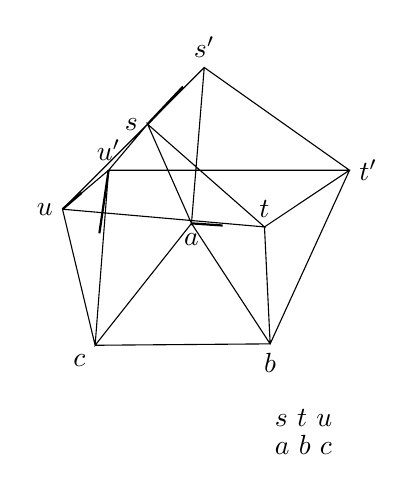
\begin{tikzpicture}[scale=.9]
\coordinate (s) at (-.7,1.6);\coordinate (sp) at (.1,2.4);\coordinate (u) at (-1.9,.4);\coordinate (up) at (-1.25,.95);\coordinate (a) at (-.08,.2);\coordinate (t) at (.95,.15);\coordinate (tp) at (2.15,.95);\coordinate (b) at (1.03,-1.5);\coordinate (c) at (-1.44,-1.52);
\draw (u)--(s)--(sp)--(tp)--(t)--(b)--(c)--(u) (sp)--(a)--(s)--(t)--(u) (up)--(tp)--(b)--(a)--(c)--(up) (u)--(up)--(s);
\draw[line width=.8pt] (s) -- +(.5,.53) (u)--+(.27,.23) (a)--+(.44,-.03) (up)--+(-.13,-.89);
\foreach \p/\l/\d in {s/s/left,sp/s'/above,u/u/left,up/u'/above,a/a/below,t/t/above,tp/t'/right,b/b/below,c/c/below left}{\node[\d] at (\p){$\l$};}
\node at (1.5,-2.55){$s\ t\ u$};\node at (1.5,-2.92){$a\ b\ c$};
\end{tikzpicture}}
\[
\begin{aligned}
x&\longmapsto y& (u\,x\,y)\\
y&\longmapsto z& (s'y,z')\\
z&\longmapsto x'&(t,z',x')
\end{aligned}
\]
\diagram{\begin{tikzcd}[ampersand replacement=\&,row sep=small,column sep=small]
\deleted{x\to y'\to z\to\unsure{x'}}\& z'\arrow[r]\&x\arrow[r,no head]\&y'\arrow[d]\\
\&y\arrow[u,no head]\&x'\arrow[l]\&z\arrow[l]
\end{tikzcd}}
\[
(a,b,c)\deleted{\unsure{\longrightarrow}}
\]
\diagram{\begin{tikzcd}[ampersand replacement=\&,row sep=tiny,column sep=small]
a\arrow[r,no head]\&b\arrow[r,no head]\&c\arrow[r]\&a\\
b\arrow[r,no head]\&a\arrow[r]\&a\arrow[r,no head]\&c\\
c\arrow[r,no head]\&c\arrow[r,no head]\&b\arrow[r]\&b
\end{tikzcd}}
\[
\boxed{\sigma_t\sigma_s\sigma_u=\deleted{\unsure{\sigma}}\sigma_{t_0}}\quad\text{sur }\widetilde E_a\deleted{\unsure{\{t_0\}}}\smallsetminus\{s,s'\}
\]
\[
\begin{aligned}
&\sigma_t\sigma_s=\sigma_{t_0}\sigma_u=\sigma_u\sigma_{t_0}\\
&\left.\begin{aligned}
&\sigma_t\sigma_s\sigma_{t\deleted{\unsure{u}}}^{-1}=\sigma_{\sigma_t s}=\sigma_u\\
&\sigma_t\sigma_s=\deleted{\unsure{\sigma_t}}\sigma_u\sigma_t\quad\text{i.e.}\quad
\underbrace{\sigma_u\sigma_t\sigma_s}_{\substack{\Vert\\\sigma_{t_0}\ \text{sur }S\smallsetminus\{t_0\}}}=\sigma_t
\end{aligned}\right\}\ \text{short-cut !!}
\end{aligned}
\]
\figure{\begin{tikzpicture}
\draw (0,0)--(.85,1)--(1.2,.08)--cycle;
\node[above right] at (.85,1){$a$};\node[left] at (0,0){$c$};\node[right] at (1.2,.08){$b$};
\node at (.9,2.1){$x\ x'$};\node at (.9,1.7){$s\ s'$};
\node at (-1.8,0){$u,u'$};\node at (-1.8,-.43){$z,z'$};
\node at (2.58,.34){$t\ t'$};\node at (2.58,-.2){$y\ y'$};
\end{tikzpicture}}
\[
\begin{aligned}
\sigma_t\sigma_y&=\sigma_y\sigma_t:\quad s\longrightarrow u\longrightarrow x\\
\sigma_u\sigma_z&=\sigma_z\sigma_u:\quad s\longrightarrow t\longrightarrow x'
\end{aligned}
\]
\scanpage{128}
% archive sheet number: 127
\unsure{+)|*)} $(S,A)$ graphe \unsure{trilitaire|trilatéraire|triangulaire} $\mathcal T_{\nu}$, avec $\deleted{\unsure{\nu>0\in\mathbb N|\nu\in\mathbb N}}\inserted{\nu=0,1\text{ ou }2}$, $c_\nu=2^\nu\geq1$

\[a\in S\]

$I$ l'ens des triangles de sommet $a$ (de cardinal $\deleted{\unsure{e}}c_\nu\inserted{+1}=2^\nu+1$)

$V$ \deleted{le groupe engendré par les $\sigma_{\underline t}$ $(\underline t\in I)$} $\deleted{\unsure{(\mathbb Z/2)^I}}\simeq\mathbb F_2^I$, il opère sur $S$ grâce aux $\sigma_{\underline t}$ $(\underline t\in I)$

$\deleted{\unsure{S|S_A}}X=\{s\in S\mid s\ \text{lié à }a\}$

\deleted{\unsure{$s\longmapsto s$|$s\longmapsto s'$}} Pour $s\in X$, on désigne par $s'$ le \deleted{\unsure{dernier}}\inserted{troisième} sommet du triangle eng. par l'arête $\{a,s\}$

Donc $s\mapsto s'$ est une involution sans pt fixe $\sigma$ de $X$, et $I\simeq X/\sigma$. On peut regarder les $X_i$ $(i\in I)$ \deleted{\unsure{soit}} comme des torseurs sous $\mathbb F_2$, donc $\prod_{i\in I}X_i$ comme un torseur sous $V$, soit $E$

\deleted{Soit} $\deleted{\unsure{E}}Y$ l'ens $S\smallsetminus X\smallsetminus\{a\}=\{\deleted{\unsure{x\in S}}\inserted{x\in S\smallsetminus\{a\}}\mid x\ \text{non lié à }a\inserted{\text{ et }a\ne}\}$

Pour tt $x\in Y$ et $i\in I$, $x$ est lié à un elt de $E_i$ et un seul, soit $\varphi_i(x)$, d'où
\[
\varphi(x)=(\varphi_i(x))_{i\in I}\in E=\prod X_i.
\]
d'où \deleted{Comment $G$ opère-t}
\[
\varphi:\ Y\longrightarrow E
\]

Comment $G$ opère-t-il (via $G\to\operatorname{Aut}(S)$.) sur $E$ ? Soit $\deleted{z\text{''}}$ \inserted{$z_0$ l'élt non nul de $\mathbb F_2$, $z$ son image \unsure{ds|de} $\mathbb F_2^I$} \deleted{l'élémt diagonal \illegible{1} de $\mathbb F_2^I$} \inserted{via l'application diagonale.} \deleted{correspond à $\unsure{t\in I}\quad\unsure{t}$ Alors $\sigma_i$ $(i\in I)$}

soit $\varepsilon_i:\mathbb F_2\longrightarrow V\simeq\mathbb F_2^I$ \deleted{\unsure{défini}} l'inj. canonique, $\rho$ l'op. naturelle \deleted{de} $V$ sur $E$ par $\rho\varepsilon_i(z_0):(x_j)_j=(y_j)_j$ avec $y_j=x_j$ si $j\ne i$, $y_j=\unsure{\varepsilon_0|z_0}x_j$ sinon. On aura alors $\deleted{\sigma_t(x)=}$
\scanpage{129}
% archive sheet number: 128
pour $x\in E=\prod_{i\in I} X_i$, \deleted{et $g=(g_i)_{i\in I}\in V$}\inserted{et $i_0\in I$}
\[
\begin{aligned}
(\sigma_{i_0})_E\deleted{\unsure{(x)=}}&=\prod_{i\in I\smallsetminus\{i_0\}}\rho(\varepsilon_i(z_0))
=\rho\biggl(\underbrace{\sum_{i\in I\smallsetminus i_0}\varepsilon_i(z_0)}_{\unsure{z\ \varepsilon_{i_0}(z_0)|z+\varepsilon_{i_0}(z_0)}}\biggr)\\
&=\rho(z)\rho(\varepsilon_{i_0}(z_0))
\end{aligned}
\]

Donc si
\[
V\xrightarrow{\unsure{\eta|\gamma}}\mathbb F_2\qquad
(\text{on a aussi }\mathbb F_2\xrightarrow{\delta=\mathrm{diag}}V)
\]
est l'augmentation naturelle, on aura pour $g\in V$
\[
(\sigma_g)_E=\rho(g\deleted{\unsure{\rho}}+\delta\eta(g))
\]

Considérons l'application
\[
V\xrightarrow{u}V\qquad u(x)=x+\delta\eta(\deleted{\unsure{g}}x)
\]
Son noyau est formé des $x$ tels que
\[
x=\delta\eta x
\]
donc \deleted{\unsure{est contenu}}\inserted{l'unique} élément non nul possible de ce noyau est $z=\delta(z_0)$, et il reste à voir quand on a $\deleted{\unsure{\delta|z}}z=\delta\eta\deleted{\unsure{\delta}}z$ i.e. $\deleted{z_0=\eta(\delta z_0}$ (comme $z=\delta z_0$) $z_0=\eta z$ i.e. $\eta z\ne0$: c'est le cas \unsure{sss|ssi} $I$ est de cardinal impair. Or ce cardinal est $1+c_\nu=1+2^\nu$, qui est impair sauf pour $\nu=0$ (cas du pavé). \deleted{Donc} \deleted{dans ce} \unsure{a)} Si $\nu=0$, $u$ est injectif donc \uline{iso}, et \deleted{\unsure{l'image}}\inserted{les op.} de $V$ sur $E$ via $\rho$ ou via $\sigma$ se déterminent mutuellement. Or l'application $\varphi$ commute bien
\scanpage{130}
% archive sheet number: 129
aux op. $\sigma$, on trouve que l'\deleted{app}image de $Y$ dans $E$ \deleted{est} (étant \unsure{invariant|invariante} sous $V$ et non vide) est $V$ tt entier. Or $\inserted{\operatorname{card}Y=}4c_\nu=4\deleted{\unsure{2^\nu=2^2}}$ \deleted{\unsure{=}}\inserted{et} $\operatorname{card}E=\operatorname{card}V$ \deleted{\unsure{donc}} $\inserted{=2^{c_\nu+1}}=2^2=4$, donc \deleted{\unsure{pour avoir un}} $\varphi$ est bijectif.

b) Si $\nu\ne0$ i.e. $\nu=1$ ou $2$, alors \deleted{l'image} $u$ a comme noyau \deleted{Im} $\delta(\mathbb F_2)=\{0,z\}$, comme image $\operatorname{Ker}\unsure{\eta|\gamma}=V$ \deleted{\unsure{A dire vrai} \inserted{\unsure{(facile)|(faible)}} \unsure{puis} $Y$ est un \unsure{tors.}}
\scanpage{131}
% archive sheet number: 130
Graphes \unsure{pseudotrilitaires|pseudotrialitaires} en termes de triangles.

$X$ ens. (``sommets'')

\[T\subset\mathcal P_3(X)\qquad\text{(triangles)}\]

\margin{Déf : $\underline a\in\mathcal P_2(X)$ est une arête si $\exists\,\underline t\in T$, $\underline a\subset\underline t$.}
\uline{Axiomes}\quad a) $\underline t,\underline t'\in T\ \Longrightarrow\ \operatorname{card}(\underline t\cap\underline t')\ne2$

i.e. si $\unsure{t',t|t,t'}$ ont deux pts en commun, ils sont égaux ou encore : tte arête contenue dans un triangle \uline{unique}

b) Soit $\underline t\in\mathcal P_3(X)$, pour que $\underline t\in T$, il (f et) \uline{suffit} que $\forall\,\underline a\in\mathcal P_2(X)$, $\underline a\subset\underline t$, on ait $\underline a$ est une arête. Ou encore

Soient $a,b,c\in X$ distincts, \deleted{\unsure{$t,$}} $\underline t,\underline t',\underline t''\in T$ tels que $a,b\in\underline t$, $b,c\in\underline t'$, $c,a\in t''$, alors $\{a,b,c\}\in T$ [et $\underline t=\underline t'=\underline t''=\{a,b,c\}$].

c) $\forall\,\underline t\in T$ et $a\in X$, $\exists\,\underline t'\in T$ tel que $a\in\underline t'$, $\underline t\cap\underline t'\ne\varnothing$ [NB si $a\notin\underline t$, $\underline t'$ est unique\ldots)

Pour que $X$ soit un \uline{\unsure{cour|carr|conf.}}, il f. et s. qu'on ait

\inserted{d) $\forall\,a\in X$, l'ens des $\underline t\in T$ tels que $a\in\underline t$ est de cardinal 3.}

Soit $X$ un \uline{cour}, $\deleted{\unsure{T|X}}X'$ l'ens de ses \unsure{triangles|\deleted{triangles}}, $R$ la relation d'incidence. Donc $\forall\,x'\in X'$, $R\{x'\}\in\mathcal P_3(X)$, et $x'\unsure{\mapstochar\relbar|\mapsto}R\{x'\}$ de $X'$ dans $\mathcal P_3(X)$ est injectif\ldots

Mais aussi, $\forall\,x\in X$, $R\{x\}\in\mathcal P_3(X')$, et $x\mapstochar\relbar R\{x\}$ de $X$ dans $\mathcal P_3(X')$ est injectif.

Soit encore $X$ son image. Montrons que $X\subset\mathcal P_3(X')$ satisfait aux conditions a) b) c) d) précédentes
\scanpage{132}
% archive sheet number: 131
Vérifions d) : $\forall\,a'\in X'$, le nb des $x\in X$ incidents à $a'$ est bien trois\ldots

a) Soient $a,b\in X$, \inserted{$a\ne b$,} considérons les $\underline t\in X'$ incidents à $a$ et $b$ à la fois, je dis qu'il y en a 0 ou 1 (jamais 2) : clair

b) Soient $\underline t,\underline t',\underline t''\in T=X'$ \inserted{él. distincts} et $a,b,c\in X$ tels que $\underline t,\underline t'$ incidents à $a$, $\underline t',\underline t''$ inc. à $b$, $\underline t'',\underline t$ inc. à $c$, prouver que $a=b=c$ donc que $\{\underline t,\underline t',\underline t''\}$ inc. à un \unsure{$=$|même} point\ldots En effet, si on avait $b\ne a$, le triangle $\underline t''$ ne pourrait rencontrer $\underline t$, car $b$ ne serait pas lié à un autre sommet de $\underline t$ que $a$.
\figure{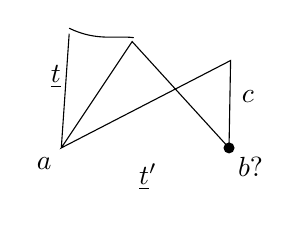
\begin{tikzpicture}
\draw (0,0)--(.1,1.45) (0.1,1.52).. controls (.45,1.35) and (.7,1.43)..(.92,1.4) (.9,1.35)--(0,0)--(2.15,1.11)--(2.13,0)--cycle;
\fill (2.13,0) circle (2pt);
\node[below left] at (0,0){$a$};\node[left] at (.12,.9){$\underline t$};\node[below] at (1.1,-.08){$\underline t'$};\node[right] at (2.17,.65){$c$};\node[below right] at (2.12,0){$b$?};
\end{tikzpicture}}

c) $\forall\,a\in X$ et $\underline t\in T=X'$\inserted{(\unsure{obs|PS|NB} $a$ n. incidt à $\underline t$)}, $\exists\,b\in X$ incident à $\underline t$, et tel que $a,b$ sont incidents à un $=$ $\underline t'\in T=X'$
\figure{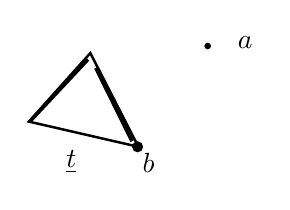
\begin{tikzpicture}
\draw[line width=.9pt] (0,0)--(.78,.87)--(1.39,-.32)--cycle;
\draw[line width=1.3pt] (.02,.01)--(.75,.79) (.85,.68)--(1.31,-.25);
\fill (1.38,-.32) circle(2pt) (2.27,.96) circle(1.2pt);
\node[right] at (2.53,1){$a$};\node[below] at (.54,-.24){$\underline t$};\node[below right] at (1.32,-.28){$b$};
\end{tikzpicture}}
\scanpage{133}
% archive sheet number: 132
\figure{\begin{tikzpicture}[scale=.72]
\foreach \x in {0,1.5,3.3}{\fill (\x,.34) circle (2.25pt) (\x+.77,.34) circle (2.25pt);\draw (\x-.06,.13).. controls (\x+.14,-.03) and (\x+.28,.23)..(\x+.42,.04)..controls(\x+.58,.14) and (\x+.63,.1)..(\x+.82,.15);}
\draw (6.45,-.22)--(7.1,.36)--(7.51,-.64)--cycle (7.57,-.75)--(8.45,-.69)--(8.49,-1.59)--cycle;
\fill (8.49,-1.59) circle(2.2pt);
\end{tikzpicture}}
\[
\lambda_{12}
\]
\figure{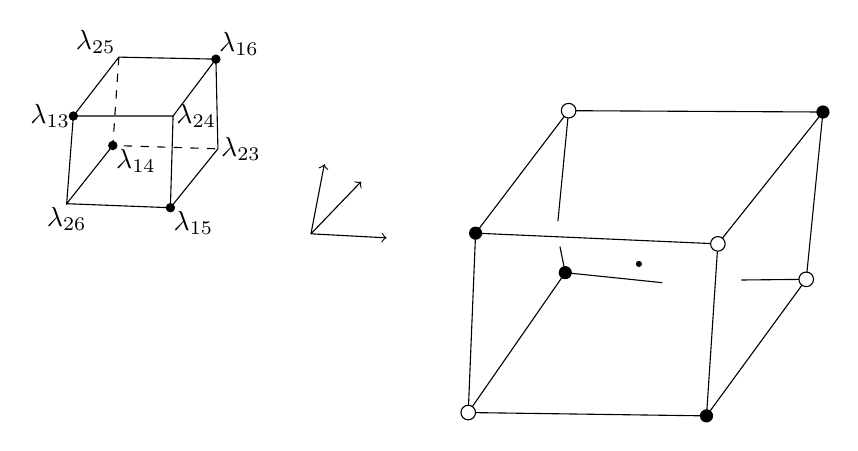
\begin{tikzpicture}[scale=.85,every node/.style={inner sep=1pt}]
\coordinate (a) at (0,0);\coordinate (b) at (1.55,-.06);\coordinate (c) at (2.26,.82);\coordinate (d) at (.69,.87);
\coordinate (e) at (.1,1.31);\coordinate (f) at (1.59,1.31);\coordinate (g) at (2.23,2.16);\coordinate (h) at (.78,2.19);
\draw (a)--(b)--(c)--(g)--(h)--(e)--(a)--(d) (e)--(f)--(g) (b)--(f);
\draw[dashed] (h)--(d)--(c);
\foreach \p in {e,b,d,g}{\fill (\p) circle(2pt);}
\node[below] at (a){$\lambda_{26}$};\node[below right] at (b){$\lambda_{15}$};\node[right] at (c){$\lambda_{23}$};\node[below right] at (d){$\lambda_{14}$};
\node[left] at (e){$\lambda_{13}$};\node[right] at (f){$\lambda_{24}$};\node[above right] at (g){$\lambda_{16}$};\node[above left] at (h){$\lambda_{25}$};
\begin{scope}[xshift=3.65cm,yshift=-.45cm]
\draw[->] (0,0)--(.2,1.04);\draw[->] (0,0)--(.75,.78);\draw[->] (0,0)--(1.13,-.06);
\end{scope}
\begin{scope}[xshift=6cm,yshift=-3.12cm]
\coordinate (a) at (0,0);\coordinate (b) at (3.56,-.05);\coordinate (c) at (5.05,1.99);\coordinate (d) at (1.45,2.09);
\coordinate (e) at (.11,2.68);\coordinate (f) at (3.73,2.52);\coordinate (g) at (5.3,4.49);\coordinate (h) at (1.5,4.51);
\draw (a)--(b)--(c)--(g)--(h)--(e)--(a)--(d) (e)--(f)--(g) (b)--(f) (h)--(1.34,2.86) (1.37,2.48)--(d)--(2.9,1.94) (4.08,1.98)--(c);
\foreach \p in {a,c,f,h}{\draw[fill=white] (\p) circle(3.1pt);}
\foreach \p in {b,d,e,g}{\fill (\p) circle(2.8pt);}
\fill (2.55,2.22) circle(1.3pt);
\end{scope}
\end{tikzpicture}}
\[
\lambda_{12}\left\{\begin{aligned}
&\lambda_{46},\lambda_{35}\\
&\lambda_{34},\lambda_{56}\\
&\lambda_{45},\lambda_{36}
\end{aligned}\right.
\]
\[
e_1+e_2/e_2+e_3/e_3+e_1
\]
\diagram{\begin{tikzcd}[ampersand replacement=\&,row sep=small]
\text{cube}\arrow[r,leftrightarrow]\&\text{cour ponctuée}\\
(\mathrm{Ens})_{2,2,2}\&(\mathrm{Ens})_2\times(\mathrm{Ens})_4\\
\unsure{\mathfrak S|\mathcal S|\mathcal G}_3.(\pm1)^3\arrow[r,phantom,"\simeq"]\&\mathfrak S_2\times\mathfrak S_4
\end{tikzcd}}
\figure{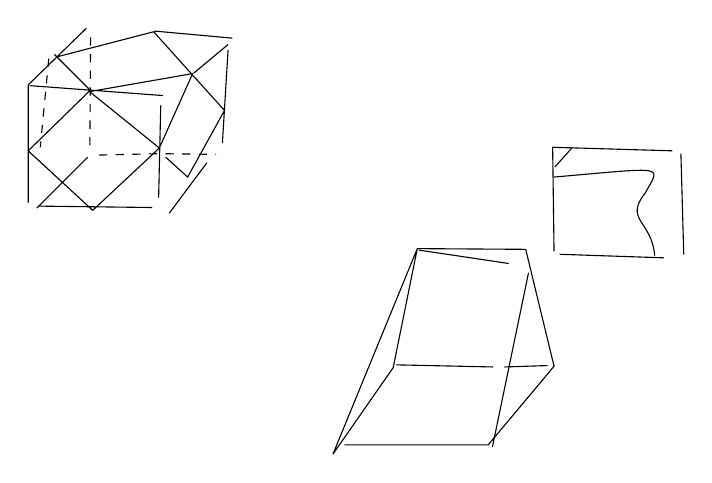
\begin{tikzpicture}[scale=.9]
\draw (0,.07)--(0,1.73)--(.82,2.53) (.02,1.72)--(1.9,1.58) (0,.8)--(.86,1.64)--(1.85,.84)--(.91,-.04)--(0,.8) (.14,.02)--(1.75,.0) (1.84,.14)--(1.87,1.44) (.37,2.16)--(.89,1.64)--(2.32,1.89)--(1.85,.84) (.42,2.13)--(1.77,2.48)--(2.3,1.89)--(2.77,1.37)--(2.25,.43)--(1.94,.71) (1.78,2.49)--(2.88,2.39) (2.34,1.9)--(2.82,2.3) (2.82,2.22)--(2.74,.91) (2.52,.63)--(1.99,-.08) (.12,-.01)--(.84,.71);
\draw[dashed,thin] (.29,2.1)--(.17,.85) (.88,2.4)--(.87,.85) (1.0,.74)--(1.85,.76)--(2.65,.75);
\begin{scope}[xshift=4.3cm,yshift=-3.48cm]
\draw (0,0)--(1.19,2.9)--(.85,1.22)--(0,0) (.16,.13)--(2.19,.13)--(3.12,1.24)--(2.72,2.89)--(1.19,2.9) (.89,1.26)--(2.26,1.23) (2.42,1.23)--(3.03,1.25);
\draw[thin] (2.76,2.56)--(2.25,.1);\draw (1.21,2.88)--(2.48,2.69);
\end{scope}
\begin{scope}[xshift=7.42cm,yshift=-.73cm]
\draw (0,.11)--(-.02,1.58)--(1.67,1.53) (1.79,1.49)--(1.83,.07) (.08,.07)--(1.55,.02);
\draw[thin] (0,1.16).. controls (1.62,1.3) and (1.5,1.33)..(1.29,.94).. controls (.98,.55) and (1.38,.55)..(1.42,.05);
\draw (.01,1.3)--(.26,1.58);
\end{scope}
\end{tikzpicture}}
\scanpage{134}
% archive sheet number: 133
$\deleted{\unsure{A_1(\mathrm{Si})|A_1(S_i)}}$

\[\left\{\begin{aligned}
&\text{diagrammes } A_2\simeq\text{triangle ponctué \deleted{\unsure{avec}}}\\
&\text{cat des graphes cubiques avec diagramme }A_2\approxeq\text{ catégorie des}\\
&\text{ensembles de cardinal 8 munis d'une involution ss pt}\\
&\text{fixe}\simeq\text{catégorie des 4-cubes}\simeq\text{catégorie des torseurs}\\
&\text{sous }\unsure{\mathfrak S|\mathcal S|\mathcal G}_4.\deleted{\mathbb Z}(\pm1)^4\simeq W_{B_4}\quad\text{(groupe de Weyl de }SO(9))
\end{aligned}\right.\]

\margin{\unsure{détermine|dilemme} pt, triangle -- pas bibase ni \unsure{tripaire|tripode}}
\figure{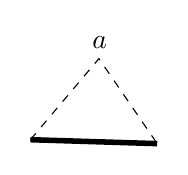
\begin{tikzpicture}
\draw[dashed] (0,0)--(.87,1.03)--(1.61,-.05);\draw[line width=2pt] (0,0)--(1.61,-.05);\node[above] at (.88,1.03){$a$};
\end{tikzpicture}}

\[\left\{\begin{aligned}
&\text{diagrammes }A_3\\
&\simeq\text{ doublet + élément de la demi-étoile associé}\\
&\simeq\text{ bibase \inserted{$B$} + él. marqué de }I=B/\sigma_B+2^{\text{ième}}\ \text{él. marqué}\\
&(\zeta_1,\lambda_{12},\zeta_1^*)\quad\text{él. typiques}\\
&\text{Cat. des graphes cubiques avec diagramme }A_2\approxeq\\
&\text{\deleted{cat des couples}}\ (\mathrm{Ens})_2\times(\mathrm{Ens})_4
\end{aligned}\right.\]

\diagram{\begin{tikzcd}[ampersand replacement=\&,column sep=large]
\zeta_1\arrow[r,no head]\&\underset{\bullet}{\lambda_{12}}\arrow[r,no head]\&\zeta_1^*
\end{tikzcd}}
\margin{détermine pt, bibase, pas triangle ni tripaire}
\figure{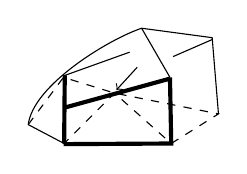
\begin{tikzpicture}[scale=.8]
\draw (0,.45).. controls (.08,1.08) and (1.27,1.8)..(1.8,1.98)--(2.92,1.83)--(3.02,.62);
\draw (2.92,1.8)--(2.3,1.53) (1.8,1.98)--(2.25,1.2) (.55,1.22)--(1.61,1.60) (0,.45)--(.57,.15);
\draw[line width=1.5pt] (.57,.15)--(.58,1.23) (.56,.14)--(2.27,.15)--(2.25,1.2) (.58,.72)--(2.25,1.18);
\draw[dashed] (0,.45)--(.56,1.2)--(1.37,.95)--(3.02,.62)--(2.27,.15)--(1.37,.95)--(.57,.15);
\draw[->] (1.73,1.36)--(1.4,1.00);
\end{tikzpicture}}

\[\left\{\begin{aligned}
&\text{diagrammes } A_4\\
&\simeq\text{pavé + triade et triangle (sécants)}\\
&\deleted{\unsure{\simeq}}\ \simeq\text{hexagone \inserted{dans pavé} + côté}\\
&\approxeq(\mathrm{Ens})_2\times(\mathrm{Ens})_3
\end{aligned}\right.\]
\figure{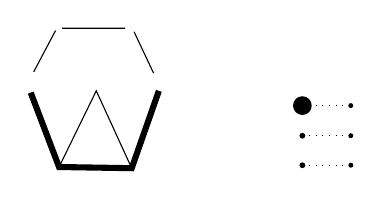
\begin{tikzpicture}[scale=.75]
\draw (0,1.23)--(.37,1.93) (.48,1.97)--(1.55,1.97) (1.7,1.91)--(2.03,1.21);
\draw[line width=2.2pt] (-.05,.88)--(.43,-.38)--(1.66,-.4)--(2.12,.91);
\draw (.43,-.38)--(1.06,.91)--(1.66,-.4);
\foreach \y in {.66,.15,-.35}{\fill (4.55,\y) circle (1.4pt) (5.37,\y) circle(1.2pt);\draw[dotted] (4.55,\y)--(5.37,\y);}
\fill (4.55,.66) circle(4.5pt);
\end{tikzpicture}}

\[\left\{\begin{aligned}
&\text{diagramme }A_5\simeq(\text{\deleted{pavé}\inserted{carré} ponctué})\\
&\hspace{5em}\simeq\text{\deleted{\unsure{carré}}\inserted{hex. ponctué}}\\
&\hspace{5em}\simeq\text{triade épinglée}\\
&\approxeq\mathrm{Ens}_{2\deleted{\unsure{,4}}}\times\mathrm{Ens}_3
\end{aligned}\right.\]
\figure{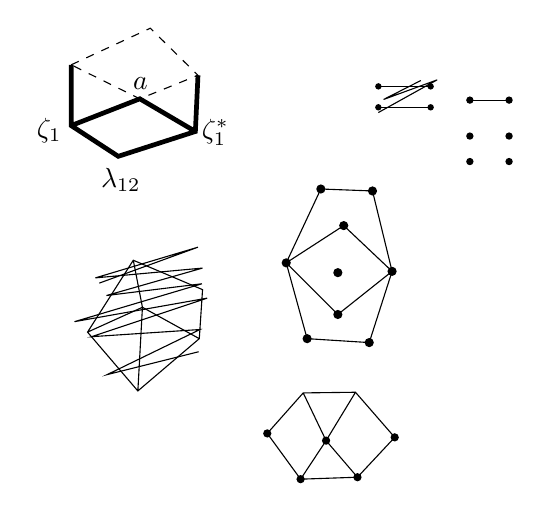
\begin{tikzpicture}[scale=.83]
\draw[line width=1.7pt] (0,1.83)--(0,.9)--(.72,.43)--(1.9,.81)--(1.94,1.67) (0,.9)--(1.05,1.31)--(1.9,.81);
\draw[dashed] (0,1.83)--(1.21,2.39)--(1.94,1.67)--(1.05,1.31)--(0,1.83);
\node[above] at (1.06,1.3){$a$};\node[left] at (0,.82){$\zeta_1$};\node[right] at (1.85,.8){$\zeta_1^*$};\node[below] at (.76,.4){$\deleted{\unsure{\lambda_{12}}}$};
\begin{scope}[xshift=4.7cm,yshift=1.18cm]
\foreach \y in {0,.32}{\draw (0,\y)--(.8,\y);\fill (0,\y) circle(1.4pt) (.8,\y) circle(1.4pt);}
\draw (0,-.08)--(.9,.42)--(.08,.12)--(.65,.41);
\draw (1.4,.11)--(2,.11);\foreach \x in {1.4,2}{\foreach \y in {.11,-.44,-.83}{\fill (\x,\y) circle(1.6pt);}}
\end{scope}
\begin{scope}[xshift=.25cm,yshift=-2.56cm]
\draw (0,.3)--(.7,1.4)--(1.76,.95)--(1.71,.2)--(.77,-.6)--cycle (0,.3)--(.84,.68)--(1.71,.2) (.77,-.6)--(.84,.68)--(.7,1.4);
\draw (.18,1.05)--(1.69,1.6)--(.12,1.13)--(1.76,1.28)--(.29,.86)--(1.75,1.04)--(-.2,.46)--(1.83,.82)--(.06,.23)--(1.72,.34)--(.3,-.35)--(1.7,.0);
\end{scope}
\begin{scope}[xshift=3.29cm,yshift=-1.5cm]
\draw (0,.3)--(.53,1.43)--(1.32,1.40)--(1.62,.17)--(1.27,-.92)--(.32,-.86)--cycle;
\draw (0,.3)--(.88,.87)--(1.62,.17)--(.79,-.49)--cycle;
\foreach \x/\y in {0/.3,.53/1.43,1.32/1.4,1.62/.17,1.27/-.92,.32/-.86,.88/.87,.79/-.49,.79/.15}{\fill (\x,\y) circle(2pt);}
\end{scope}
\begin{scope}[xshift=3cm,yshift=-4.16cm]
\draw (0,.35)--(.55,.97)--(1.35,.98)--(1.95,.29)--(1.38,-.32)--(.51,-.35)--cycle (.55,.97)--(.9,.24)--(1.38,-.32) (.51,-.35)--(.9,.24)--(1.35,.98);
\foreach \x/\y in {0/.35,.9/.24,1.95/.29,.51/-.35,1.38/-.32}{\fill (\x,\y) circle(1.8pt);}
\end{scope}
\end{tikzpicture}}
\scanpage{135}
% archive sheet number: 134
\figure{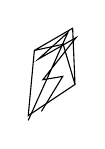
\begin{tikzpicture}[scale=.6]
\draw (0,0)--(.13,1.38)--(.94,1.85)--(.99,.66)--cycle (.13,1.38)--(.74,1.51)--(.99,.66);
\draw (0,-.1)--(.84,1.76)--(.22,1.2)--(1.01,1.65)--(.31,.76)--(.73,.83)--(.28,.09);
\end{tikzpicture}}
\[\left\{\begin{aligned}
&\text{Prismes triangulaires \deleted{\unsure{dans}} pavé + triangles}\\
&\approxeq(\mathrm{Ens})_2\times(\mathrm{Ens})_3\times(\mathrm{Ens})_3
\end{aligned}\right.\]

\noindent\rule{.33\linewidth}{.4pt}
\figure{\begin{tikzpicture}[scale=.75,every node/.style={inner sep=1pt}]
\draw (0,3.95)--(.01,5.45)--(1.53,5.48)--(1.45,3.87)--cycle (.01,5.45)--(.65,6.07)--(2.28,6.07)--(2.11,4.79) (0,3.95)--(.69,4.75)--(1.95,4.73) (1.53,5.48)--(2.28,6.07) (.65,6.07)--(.69,4.75);
\draw (.06,5.3)..controls (2.63,7.33) and (2.16,6.32)..(.32,5.12)..controls (.03,4.73) and (2.62,6.29)..(1.55,5.03)..controls (.59,3.97) and (2.02,3.99)..(1.84,3.99);
\draw (.66,5.11)..controls (1.85,5.37) and (.86,4.47)..(.86,4.09)..controls(.86,3.95) and (1.21,3.94)..(1.34,3.95);
\begin{scope}[xshift=1.13cm,yshift=2.13cm]
\draw (0,0)--(0,1.09)--(1.52,1.17)--(1.55,.05)--cycle (1.55,.05)--(2.96,.03)--(3,1.24)--(1.52,1.17)--(1.81,1.55)--(1.79,2.26)--(2.98,1.25) (0,1.09)--(1.79,2.26)--(.06,.05) (1.79,2.26)--(2.85,.10);
\fill (.83,.55) circle(1.5pt) (2.22,.58) circle(1.5pt);
\draw[->] (-.76,.91)--(3.09,1.99);\draw (-.22,-.3)--(5.81,1.86);
\coordinate (s) at (2.49,0);\node[above left] at (s){$s$};\fill (s) circle(1.7pt);
\draw (s)--(3.39,.59);\node[above right] at (3.39,.59){$u$};
\draw (1.07,-.86)--(3.42,-.85)--(3.47,-1.79)--(1.14,-1.78)--cycle (1.07,-.86)--(s)--(3.42,-.85) (1.14,-1.78)--(s)--(3.39,-1.72) (s)--(2.57,-.60)--(2.22,-1.78) (2.22,-.85)--(2.22,-1.78);
\node[left] at (1.07,-.88){$a'$};\node[right] at (3.42,-.82){$a''$};\node[left] at (2.34,-.65){$a$};\node[right] at (2.57,-.6){$t$};
\node[below left] at (1.14,-1.78){$b'$};\node[below] at (2.22,-1.78){$b$};\node[below right] at (3.42,-1.78){$b''$};
\node at (4.98,.78){$\deleted{\text{bicarré}}$};
\draw (s)--(11.84,2.0);
\draw[thin] (-.91,1.55)..controls (-1.13,.87) and (-.76,-.4)..(-1.39,-.35)..controls(-.92,-.28) and (-1.08,-1.16)..(-.84,-1.88);
\end{scope}
\begin{scope}[xshift=11.24cm,yshift=2.68cm]
\draw (0,0)--(-.03,.93)--(1.42,.98)--(1.48,-.03)--cycle (1.48,-.03)--(2.86,.03)--(2.76,.97)--(1.42,.98);
\draw (0,.95)--(1.6,1.95)--(2.76,.97) (0,.04)--(1.6,1.95)--(1.48,-.03) (0,.04)--(.61,-.95)--(1.48,-.03)--(2.18,-.96)--(2.86,.03) (1.6,1.95)--(2.86,.03) (2.76,.97)--(2.17,-.38) (.61,-.95)--(.82,.42)--(1.63,1.19) (0,.95)--(.62,-.39)--(1.6,1.95);
\draw[line width=1pt] (1.48,-.03)--(1.42,.98)--(1.63,1.19);
\fill (2.09,.43) circle(1.5pt);
\end{scope}
\end{tikzpicture}}

les triangles sur $(a'b')$ et $(a''b'')$ ont $=$ sommet $s$

Si $t$ est le \inserted{$3^e$ sommet du} triangle de base $(a,b)$, le \deleted{\unsure{centre de|cube de}} troisième sommet \inserted{$u$} du triangle de base $(st)$ est le centre du \inserted{\unsure{carr|carré}} $(abb'a')$ et du carré $(abb''a'')$. Donc les deux carré ont $=$ centre\inserted{$u$}, et étant distincts, ne sont pas contenus dans le $=$ pavé -- ils engendrent donc une \unsure{cour.} On peut dire aussi que
\figure{\begin{tikzpicture}[scale=.8]
\fill (-1.4,1.26) circle(3pt);
\draw[gray] (.6,1.62)--(.85,.53)--(1.9,.52)--(2.23,1.51) (3.63,3.88)--(3.66,2.91)--(5.17,2.92)--(5.2,3.91);
\draw (0,0)--(1.57,-.02) (1.72,-.01)--(3.1,-.06)--(3.03,-1)--(3.69,-.65) (0,0)--(0,-.96)--(.44,-.99);
\draw[dashed] (0,-.96)--(1.28,-2.26)--(3.03,-1) (3.68,.03)--(3.69,-.65);
\fill (1.57,-.02) circle(1.8pt) (3.1,-.06) circle(1.7pt) (1.28,-2.26) circle(1.6pt);
\node[above left] at (0,0){$a'$};\node[above] at (1.57,-.02){$\deleted{\unsure{c}}a$};\node[above] at (3.69,.04){$\unsure{a'|a''}$};\node[below left] at (0,-1){$b'$};\node[below] at (3.56,-.73){$b''$};
\end{tikzpicture}}
est un $A_5$ contenu dans un pavé unique, en fait c'est un hexagone \unsure{épointé|épinglé|ponctué} de façon unique en désignant la triade $(d,b',b'')$ -- et il faut choisir un pt $b$ lié aux trois pts de cette triade, i.e. appartenant à la triade \unsure{opposée|apposée}

Card des choix au total $\tfrac12(720\times6\times3)=2^{\unsure{4}}.3^4.5=N:2^3$ -- en effet, la cat. des \deleted{\illegible{1}} graphes cubiques avec bicarré est
\[
\simeq\underbrace{(\mathrm{Ens})_2\times(\mathrm{Ens})_2}_{\text{bicarré}}\times
\underbrace{(\mathrm{Ens})_2}_{\substack{\text{compléter l'enveloppe}\\\text{quasi-trilitaire en}}}
\simeq\operatorname{Tors}((\pm1)^3)
\]
\scanpage{136}
% archive sheet number: 135
\figure{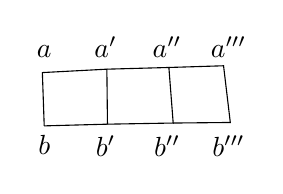
\begin{tikzpicture}[x=.78cm,y=.72cm]
\draw (0,0)--(-.03,.94)--(1.02,1)--(1.03,.03)--(0,0);
\draw (1.02,1)--(2.03,1.03)--(2.10,.05)--(1.03,.03);
\draw (2.03,1.03)--(2.92,1.06)--(3.03,.06)--(2.10,.05);
\foreach \x/\t/\b in {0/a/b,1/{a'}/{b'},2/{a''}/{b''},3/{a'''}/{b'''}}{
\node[above] at (\x,1.03){$\t$};\node[below] at (\x,0){$\b$};}
\end{tikzpicture}}
n'existe pas dans graphe cubique, car on trouve que les \deleted{triangles de bases}\inserted{$3^{\mathrm e}$ sommet} des triangles de bases $(a''',b''')$ égale celui du triangle de bases $(a^{\deleted{\unsure{''}}},b^{\deleted{\unsure{'|''}}})$ et $(a^{\deleted{\unsure{''|'}}},b')$, ce qui sont donc égaux -- absurde d'après étude du carré

Conséquence : pas de prismes à bases pentagonale et hexagonale. Par contre $\unsure{\exists|\nexists}$ prismes à base carré, i.e. cubes.

\margin{\uline{NB} : Carré définit pt, \unsure{paire de tripaires|paire de triplets|paire de tripodes}, une bibase, un triangle\ldots}

Carrés de centre un pt donné $a$ : d'abord la \deleted{\unsure{cat.}}donnée des graphes cubiques à pt marqué $a$, équivaut à celle d'un ens $I$ de card. $5$ et d'un torseur $T$ sous $V_I=(\mathbb F_2^I)'$ \inserted{(de dim $4$ sur $\mathbb F_2$)} engendré par des $e_i$ $(i\in I)$ avec la seule relation $\sum e_i=0$. L'ens des pts non liés à $a$ est $T$. Les \deleted{\unsure{de|donnée}} carrés sont les sous-espaces affines de dim $2$, dont l'espace des translations soit engendrés par $2$ parmi les $e_i$, \deleted{\unsure{donc}}\inserted{corr.} à une partie $I'$ de $I$ de cardinal $2$. Si $V_{(I')}$ est le sous-vectoriel correspondant, les carrés en question correspondent aux pts de $T/V_{(I')}$, ou aux restrictions du groupe structural de $V_I$ à $V_{(I')}\simeq\mathbb F_2^{I'}$. $[$Donc la cat. des graphes cubiques $+$ carrés équivaut à celle des \deleted{couples}\inserted{triplets} \deleted{$(\unsure{I'},\unsure{T'})$} $(\unsure{I'|I''}$ ens. de card. $2$, $T'$ torseur sous $\mathbb F_2^{I'}$, $I''(=I\backslash I')$ ens de card. $3)$ i.e. $(\mathrm{Ens})_{2,2}\times\mathrm{Ens}_3\simeq\text{Carré}\times(\mathrm{Ens})_3$
